\chapter{Implementation}

\textbf{Author: } 

\section{Generating test data}
Good test data is of utmost importance in machine learning. The system can only know information that is depicted in the training data, which is why it is important to include as many aspects of the problem as possible in this data.

Since machine learning needs a lot of data in order to solve the given task it can be tiresome to generate and label all this data by hand. Therefore the authors decided to simulate the objects and the camera using a computer graphics modelling software called Blender.

Blender allows for relatively easy generation of training data by providing a Python API.

[TODO: Image camera setup, lightning, objects in Blender]

[TODO: Renders and labels for example objects]

\section{OpenCV}
OpenCV is a framework for image manipulation. Some of its use cases are changing the colour spectrum, filtering the image by colour and cropping images. The authors use OpenCV to test whether there are differences between filters for the images in the training data, for example greyscale images compared to coloured images.

[TODO: image manipulation und ...; aka besser beschreiben was OpenCV ist]

[TODO: wofür verwenden wir es? Ergebnisse zw. Graustufen und Farbbildern]

[TODO: Codebeispiele?]

\subsection{Greyscale}

\begin{figure}[h!]
	\centering
	%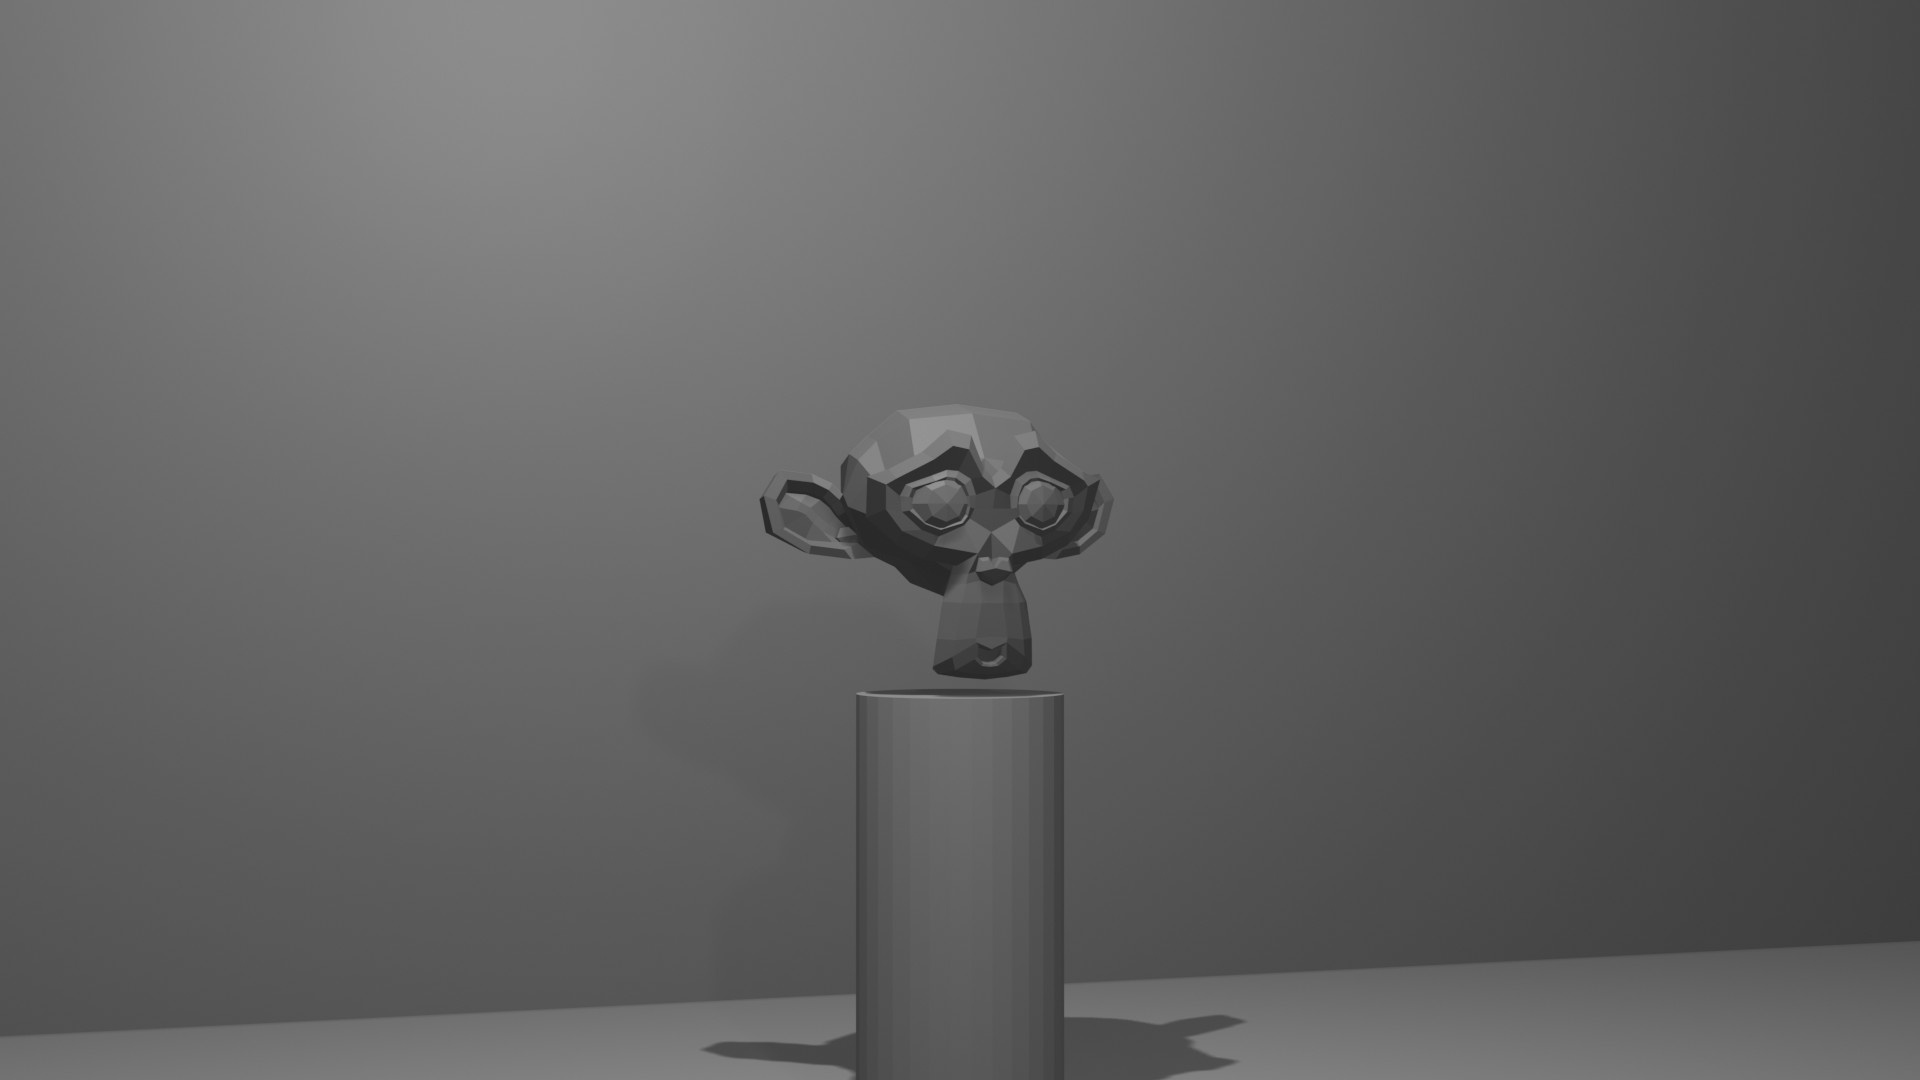
\includegraphics[width=4.5in]{img/implementation_opencv_greyscale.png}
	\caption{Comparison between normal and greyscale image.}
	\label{pic:implementation_opencv_greyscale}
\end{figure}

\subsection{Saturated}

\begin{figure}[h!]
	\centering
	%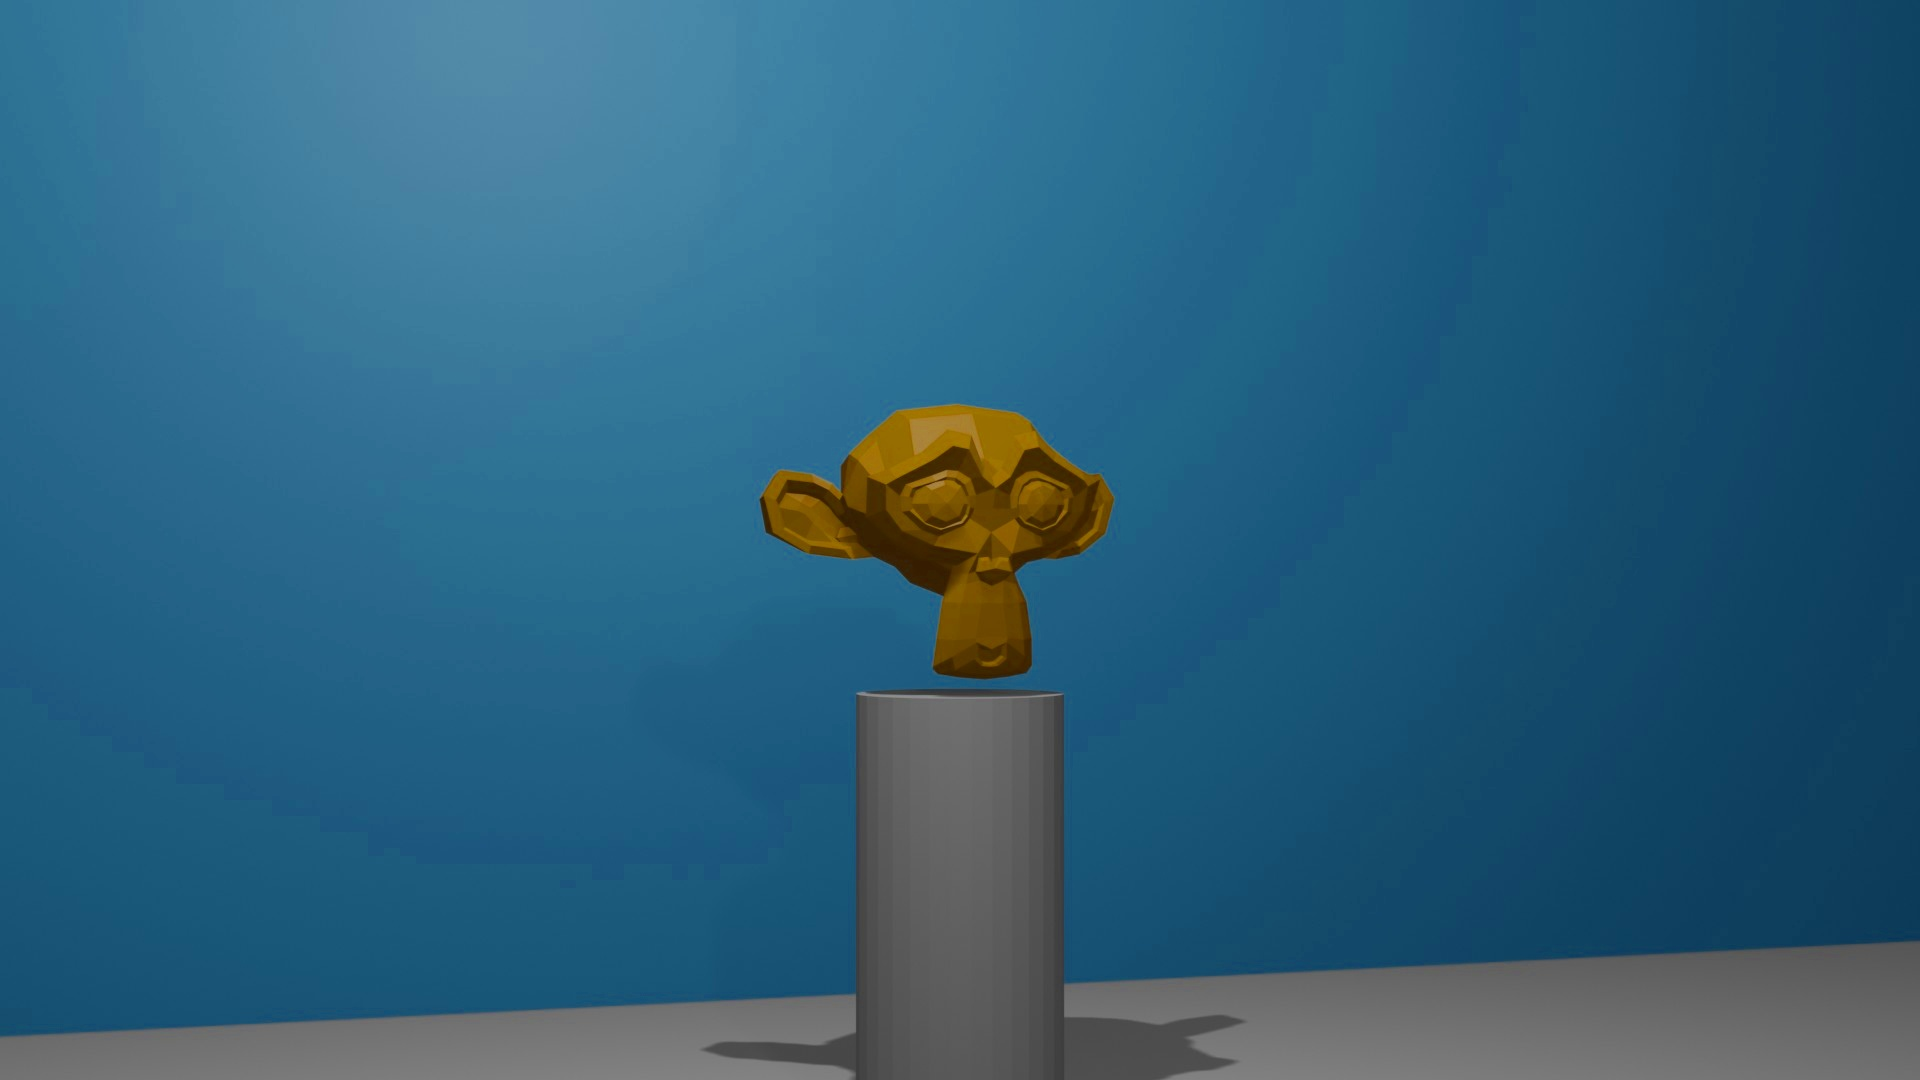
\includegraphics[width=4.5in]{img/implementation_opencv_saturated.png}
	\caption{Comparison between normal and saturated image.}
	\label{pic:implementation_opencv_saturated}
\end{figure}

\subsection{Resolution}

\begin{figure}[h!]
	\centering
	%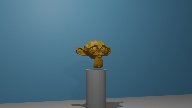
\includegraphics[width=4.5in]{img/implementation_opencv_resolution.png}
	\caption{Comparison between normal and resolution image.}
	\label{pic:implementation_opencv_resolution}
\end{figure}

\subsection{Brightness}

\begin{figure}[h!]
	\centering
	%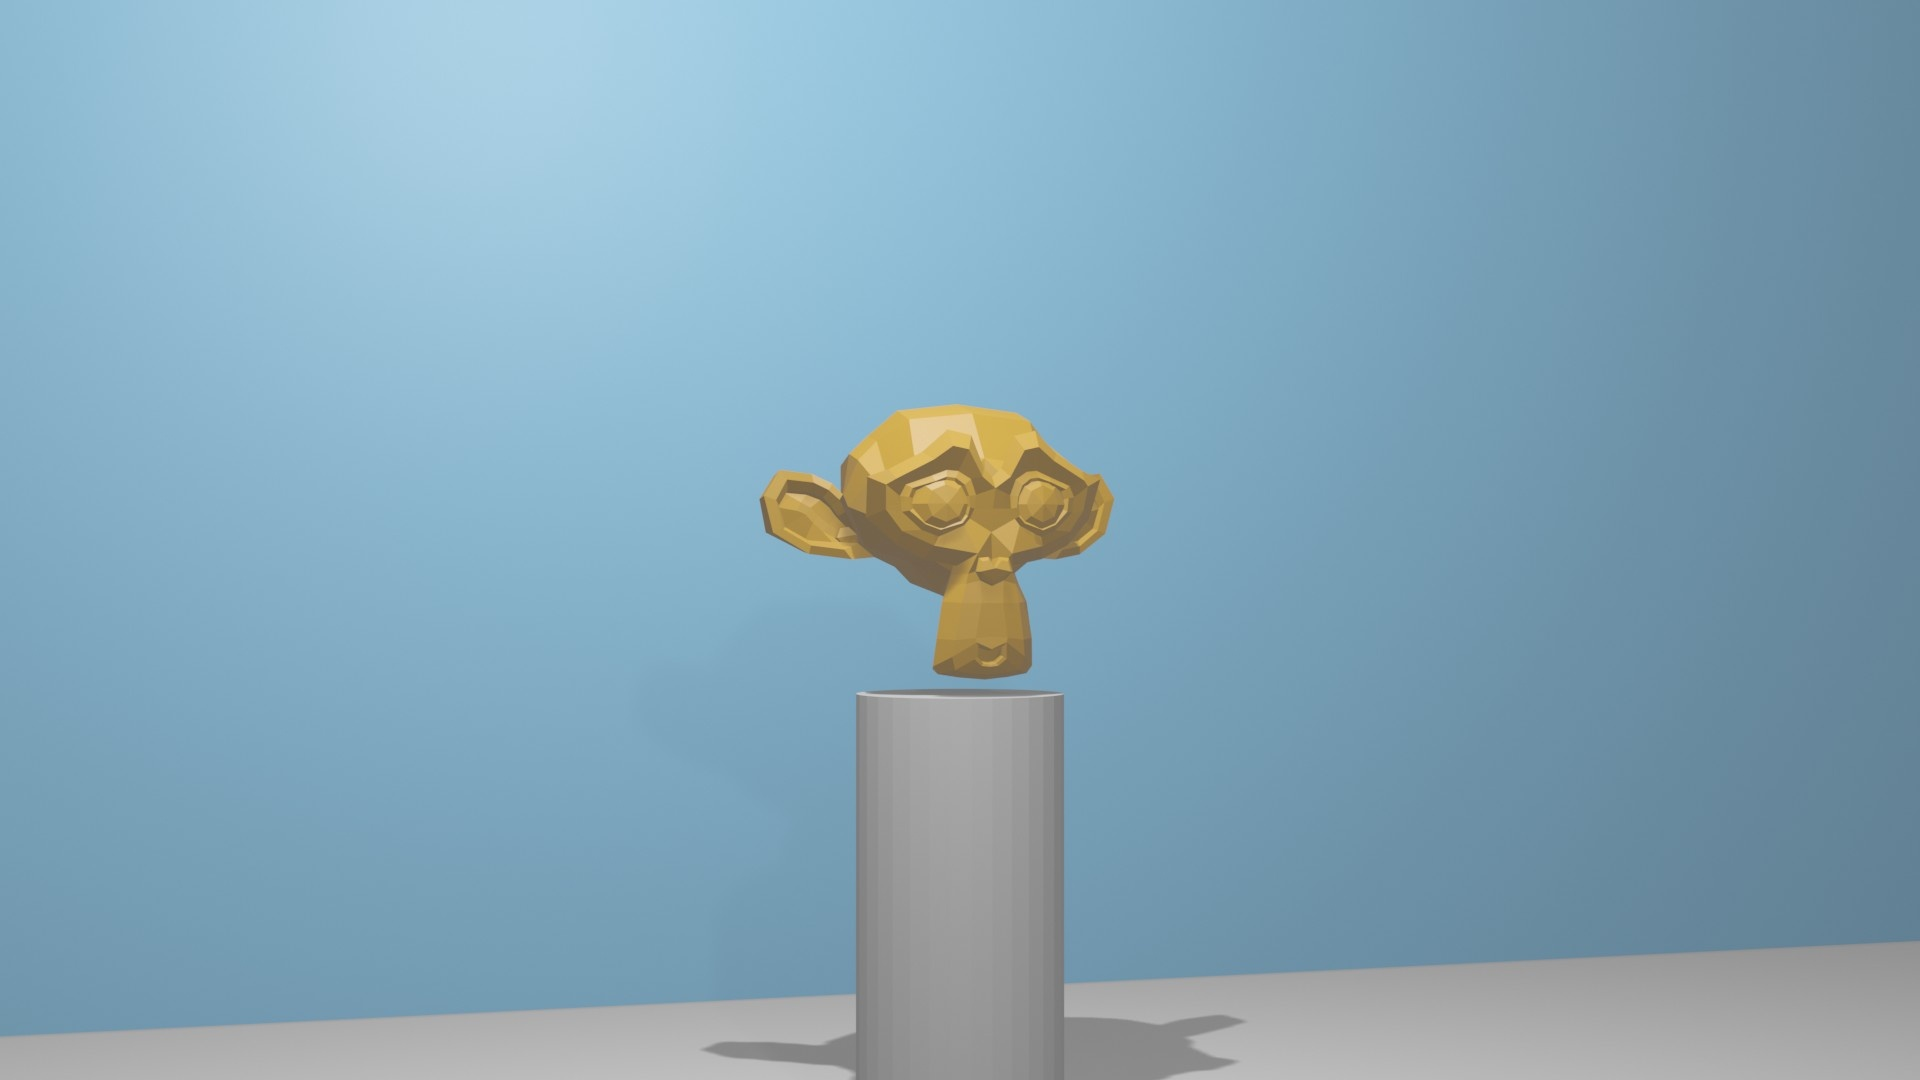
\includegraphics[width=4.5in]{img/implementation_opencv_brightness.png}
	\caption{Comparison between normal and brightness image.}
	\label{pic:implementation_opencv_brightness}
\end{figure}

\section{Neural Network}
The authors decided to use a software framework called TensorFlow for the first implementation of the neural network. This has the following two advantages: using Tensorflow allows for a low effort proof of concept and it makes testing out different configurations (e.g. number of hidden layers or filters in image preprocessing) of the neural network easier.

After it has been shown that the challenge of detecting the distance to an object can be solved using machine learning, the authors plan on implementing a neural network in C++ on their own. The knowledge gained in the TensorFlow implementation will be used in the C++ implementation, which hopefully will make the work less time consuming.

\section{TensorFlow}
As machine learning has gained popularity in recent years the demand for applicable frameworks grew. One of the most popular is called TensorFlow. It was developed by Google for internal use and was published under the Apache License 2.0 on the \nth{9} of November 2015.

TensorFlow supports APIs for Python, C, C++, Go, Java, JavaScript and Swift.
Due to its popularity third party APIs for C\#, R, Scala, Rust and many more were developed.

Its use cases reach from categorizing handwritten digits to YouTube video recommendations, one of the many applications Google use it for.

Tom Hope et al. describe TensorFlow as a software framework for numerical computations based on dataflow graphs \footcite[page 6]{Hope_Learning_TensorFlow}.

\subsection{Computation graph}
To compute a value using TensorFlow a computation graph has to be constructed. In this graph each node corresponds to an operation, such as subtraction or division. By connecting these nodes via edges the output of one node can be fed as input into another node. One example of such a computation graph can be seen in Figure~\ref{pic:implementation_tensorflow_nodesAndGraphs_computationGraph}.

\begin{figure}[h!]
	\centering
	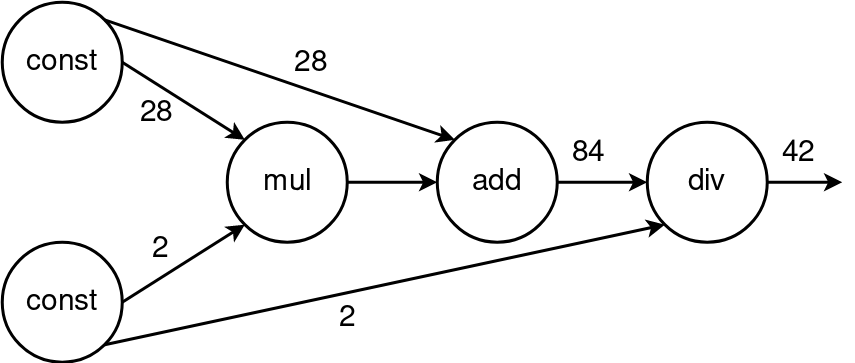
\includegraphics[width=4.5in]{img/implementation_tensorflow_nodesAndGraphs_computationGraph.png}
	\caption{Each node represents an operation, where $const$ stands for a constant value, $add$ for addition, $mul$ for multiplication and $div$ for division. Edges, represented by arrows, connect nodes. The information shared between the nodes is described by the numbers written next to the edges. This computational graph calculates the result of the arithmetic expression $(28 * 2) + 28 / 2$.}
	\label{pic:implementation_tensorflow_nodesAndGraphs_computationGraph}
\end{figure}

The implementation of the computation graph, shown in Figure~\ref{pic:implementation_tensorflow_nodesAndGraphs_computationGraph}, in Python could look as follows:

\begin{lstlisting}[language=python]
import tensorflow as tf

a = tf.constant(28)
b = tf.constant(2)

c = tf.multiply(a, b)
d = tf.add(a, c)
e = tf.divide(d, b)

with tf.Session() as sess:
    out = sess.run(e)

print(out)

\end{lstlisting}

The first line specifies that the TensorFlow functionality should be imported. Line 3 and 4 define the two constant values and assigns them the values 28 and 2 respectively. In line 6 to 8 the other nodes of the graph are specified. E.g. in line 6 a new node, named $c$, is created and the output of node $a$ and node $b$ are connected as its input. To perform the calculation described by the graph a new session is created in line 10. Finally the output of the graph (node $e$) is specified in line 11, the result is calculated and printed in line 13.

TensorFlow allows for another way of specifying a graph with these arithmetic operations:

\begin{lstlisting}[language=python]
import tensorflow as tf

a = tf.constant(28)
b = tf.constant(2)

e = (a * b + a) / b

with tf.Session() as sess:
	out = sess.run(e)

print(out)

\end{lstlisting}

This code is equivalent to the first one, but uses syntactic sugar to shorten line 6 to 8 in the first code block into line 6. At this point it should be noted that while it might look like it line 6 does not calculate anything. It simply describes how the computational graph should look. The answer (42) is calculated in the session in line 9.

\subsection{Convonutional Neural Networks?}

\subsection{Alternatives to Tensorflow}
[INFO: Abstraction libraries such as Keras and TF-Slim offer simplified  high-level  access  to  the  "LEGO  bricks"  in  the  lower-level  library,  helping  to streamline the construction of the dataflow graphs, training them, and running inference. \footcite[page 7]{Hope_Learning_TensorFlow}]

\begin{center}
\begin{tabular}{| l | l | l | l | l |}
	\hline
	\bfseries & \bfseries Open Source & \bfseries Actively & \bfseries Parallelization & \bfseries Interface \\
	 & & \bfseries developed & & \\
	\hline
	\bfseries TensorFlow & Yes & Yes & Yes & Python, C, C++, \\
	& & & & Go, Java, JavaScript, \\
	& & & & Swift, R, Julia \\
	\hline
	\bfseries Keras & Yes & Yes & Yes & Python \\
	\hline
	\bfseries PyTorch & Yes & Yes & Yes & Python, C++ \\
	\hline
	\bfseries Torch & Yes & No & Yes & Lua, LuaJIT, C, \\
	& & & & C++, OpenGL \\
	\hline
	\bfseries Wolfram & No & Yes & Yes & Wolfram Language \\
	\bfseries Mathematica & & & & \\
	\hline
\end{tabular}
\label{tab:implementation_tensorflow_alternativesToTensorflow_comparision}
\end{center}

[+ warum verwenden wir ausgerechnet Tenserflow]

\subsection{Structure of our Neural Network}

[wie lesen wir Daten ein, wie viele layer, was ist der output (maximale entfernung? z.B. 10m)]

\section{C++ Implementation}

\section{Technical difficulties}

\filbreak